\section{User Interface Components}
\subsection{Landing Page}
\begin{figure}[H]
    \centering
    \includegraphics[width=0.8\textwidth]{images/hm-landing-new.png}
    \caption{HealthHub Landing Page Implementation}
\end{figure}

The landing page implementation from our codebase:
\begin{lstlisting}[language=TypeScript, caption=Landing Page Implementation]
// app/(app)/about/page.tsx
export default function AboutPage() {
    return (
        <div className="flex flex-col items-center justify-center min-h-screen">
            <section className="hero-section">
                <h1>HealthHub: Comprehensive Health Monitoring</h1>
                <p>AI-powered health data management and analysis</p>
            </section>
        </div>
    );
}
\end{lstlisting}

\section{AI Implementation}
\subsection{RAG Pipeline}
Implementation of the RAG query system:
\begin{lstlisting}[language=TypeScript, caption=RAG Query Implementation]
// app/api/rag-query/route.ts
export async function POST(req: Request) {
    try {
        const { query, userId } = await req.json();
        const supabase = createRouteHandlerClient({ cookies });
        
        // Fetch user's health records
        const { data: documents } = await supabase
            .from('health_records')
            .select('content, metadata')
            .eq('user_id', userId);
            
        // Generate embeddings and find relevant context
        const relevant_docs = await getRelevantDocuments(query, documents);
        
        return NextResponse.json({ response });
    } catch (error) {
        return NextResponse.json(
            { error: "Failed to process query" },
            { status: 500 }
        );
    }
}
\end{lstlisting}

\subsection{Chat Interface}
\begin{figure}[H]
    \centering
    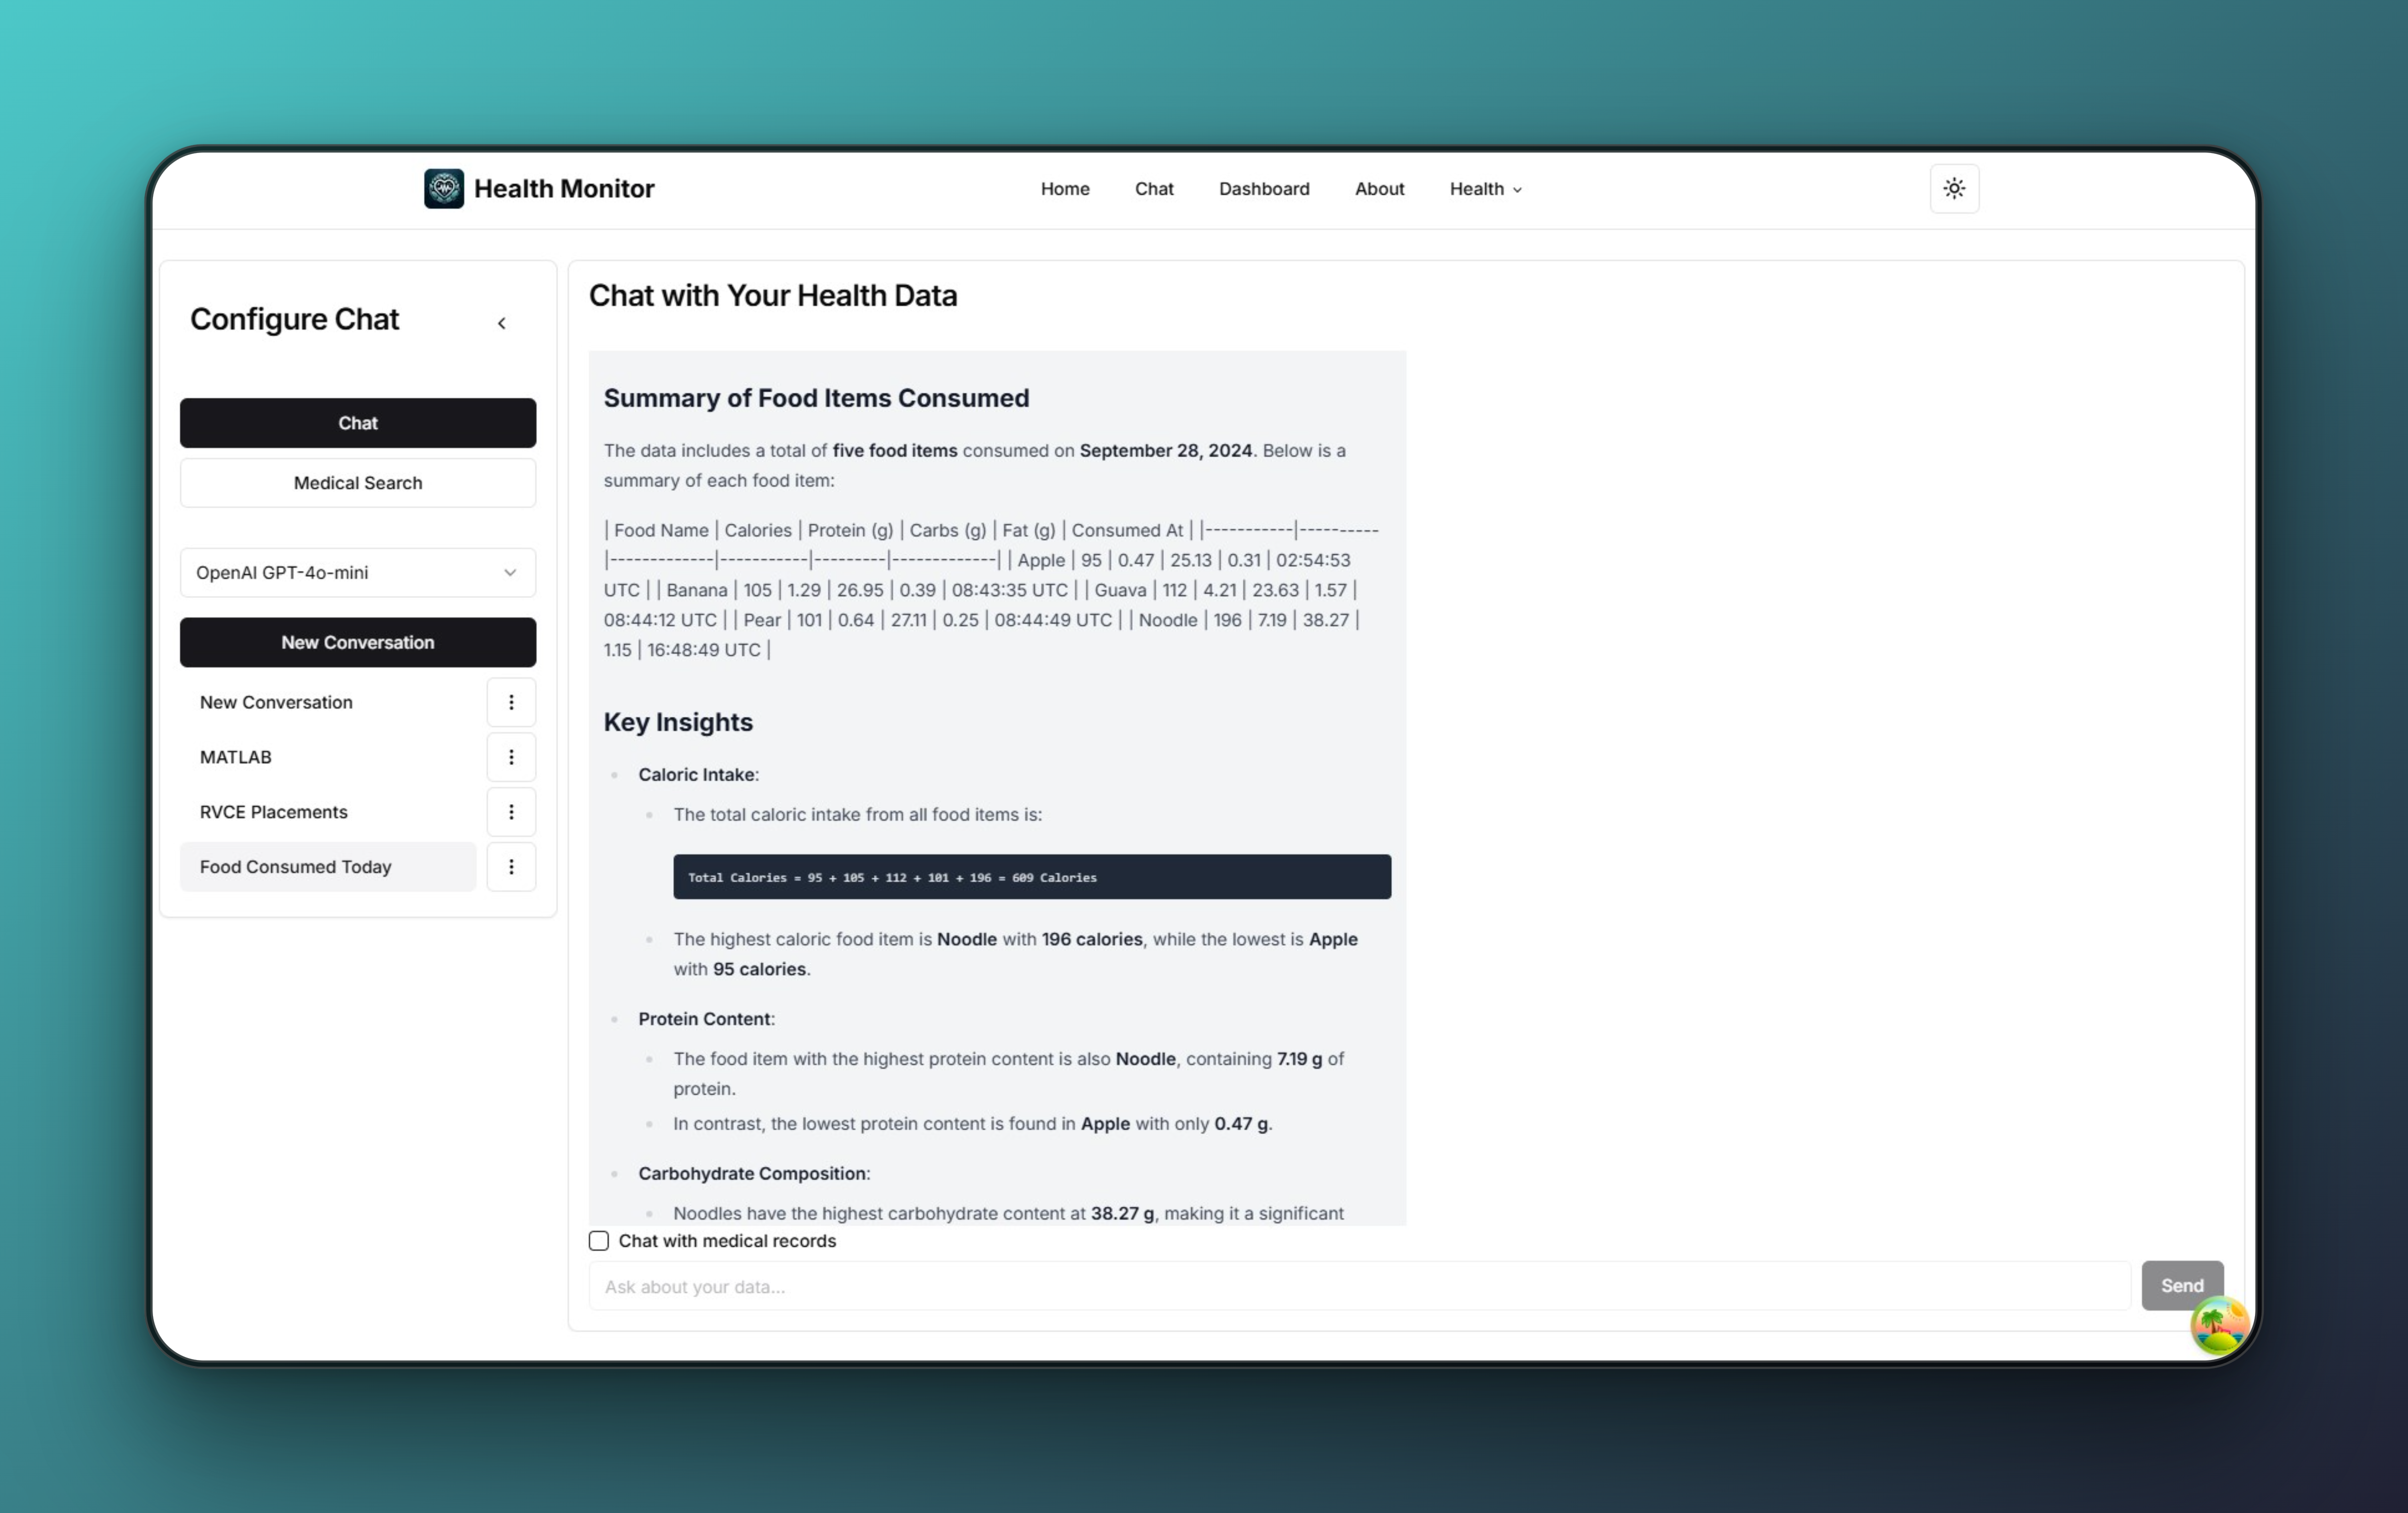
\includegraphics[width=0.8\textwidth]{images/hm-chat-light.png}
    \caption{AI Health Assistant Implementation}
\end{figure}

Chat interface implementation:
\begin{lstlisting}[language=TypeScript, caption=Chat Implementation]
// app/(chat)/chat/ChatPageClient.tsx
export default function ChatPageClient() {
    const [messages, setMessages] = useState<Message[]>([]);
    const [input, setInput] = useState('');

    const handleSubmit = async (e: React.FormEvent) => {
        e.preventDefault();
        if (!input.trim()) return;

        const userMessage = { role: 'user', content: input };
        setMessages(prev => [...prev, userMessage]);
        setInput('');

        try {
            const response = await fetch('/api/chat', {
                method: 'POST',
                body: JSON.stringify({ messages: [...messages, userMessage] })
            });
        } catch (error) {
            console.error('Failed to get response:', error);
        }
    };

    return (
        <div className="chat-container">
            <div className="messages-container">
                {messages.map((msg, idx) => (
                    <MessageComponent key={idx} message={msg} />
                ))}
            </div>
            <form onSubmit={handleSubmit}>
                <input
                    value={input}
                    onChange={(e) => setInput(e.target.value)}
                    placeholder="Ask about your health..."
                />
                <button type="submit">Send</button>
            </form>
        </div>
    );
}
\end{lstlisting}

\section{Data Visualization}
\subsection{Analytics Dashboard}
\begin{figure}[H]
    \centering
    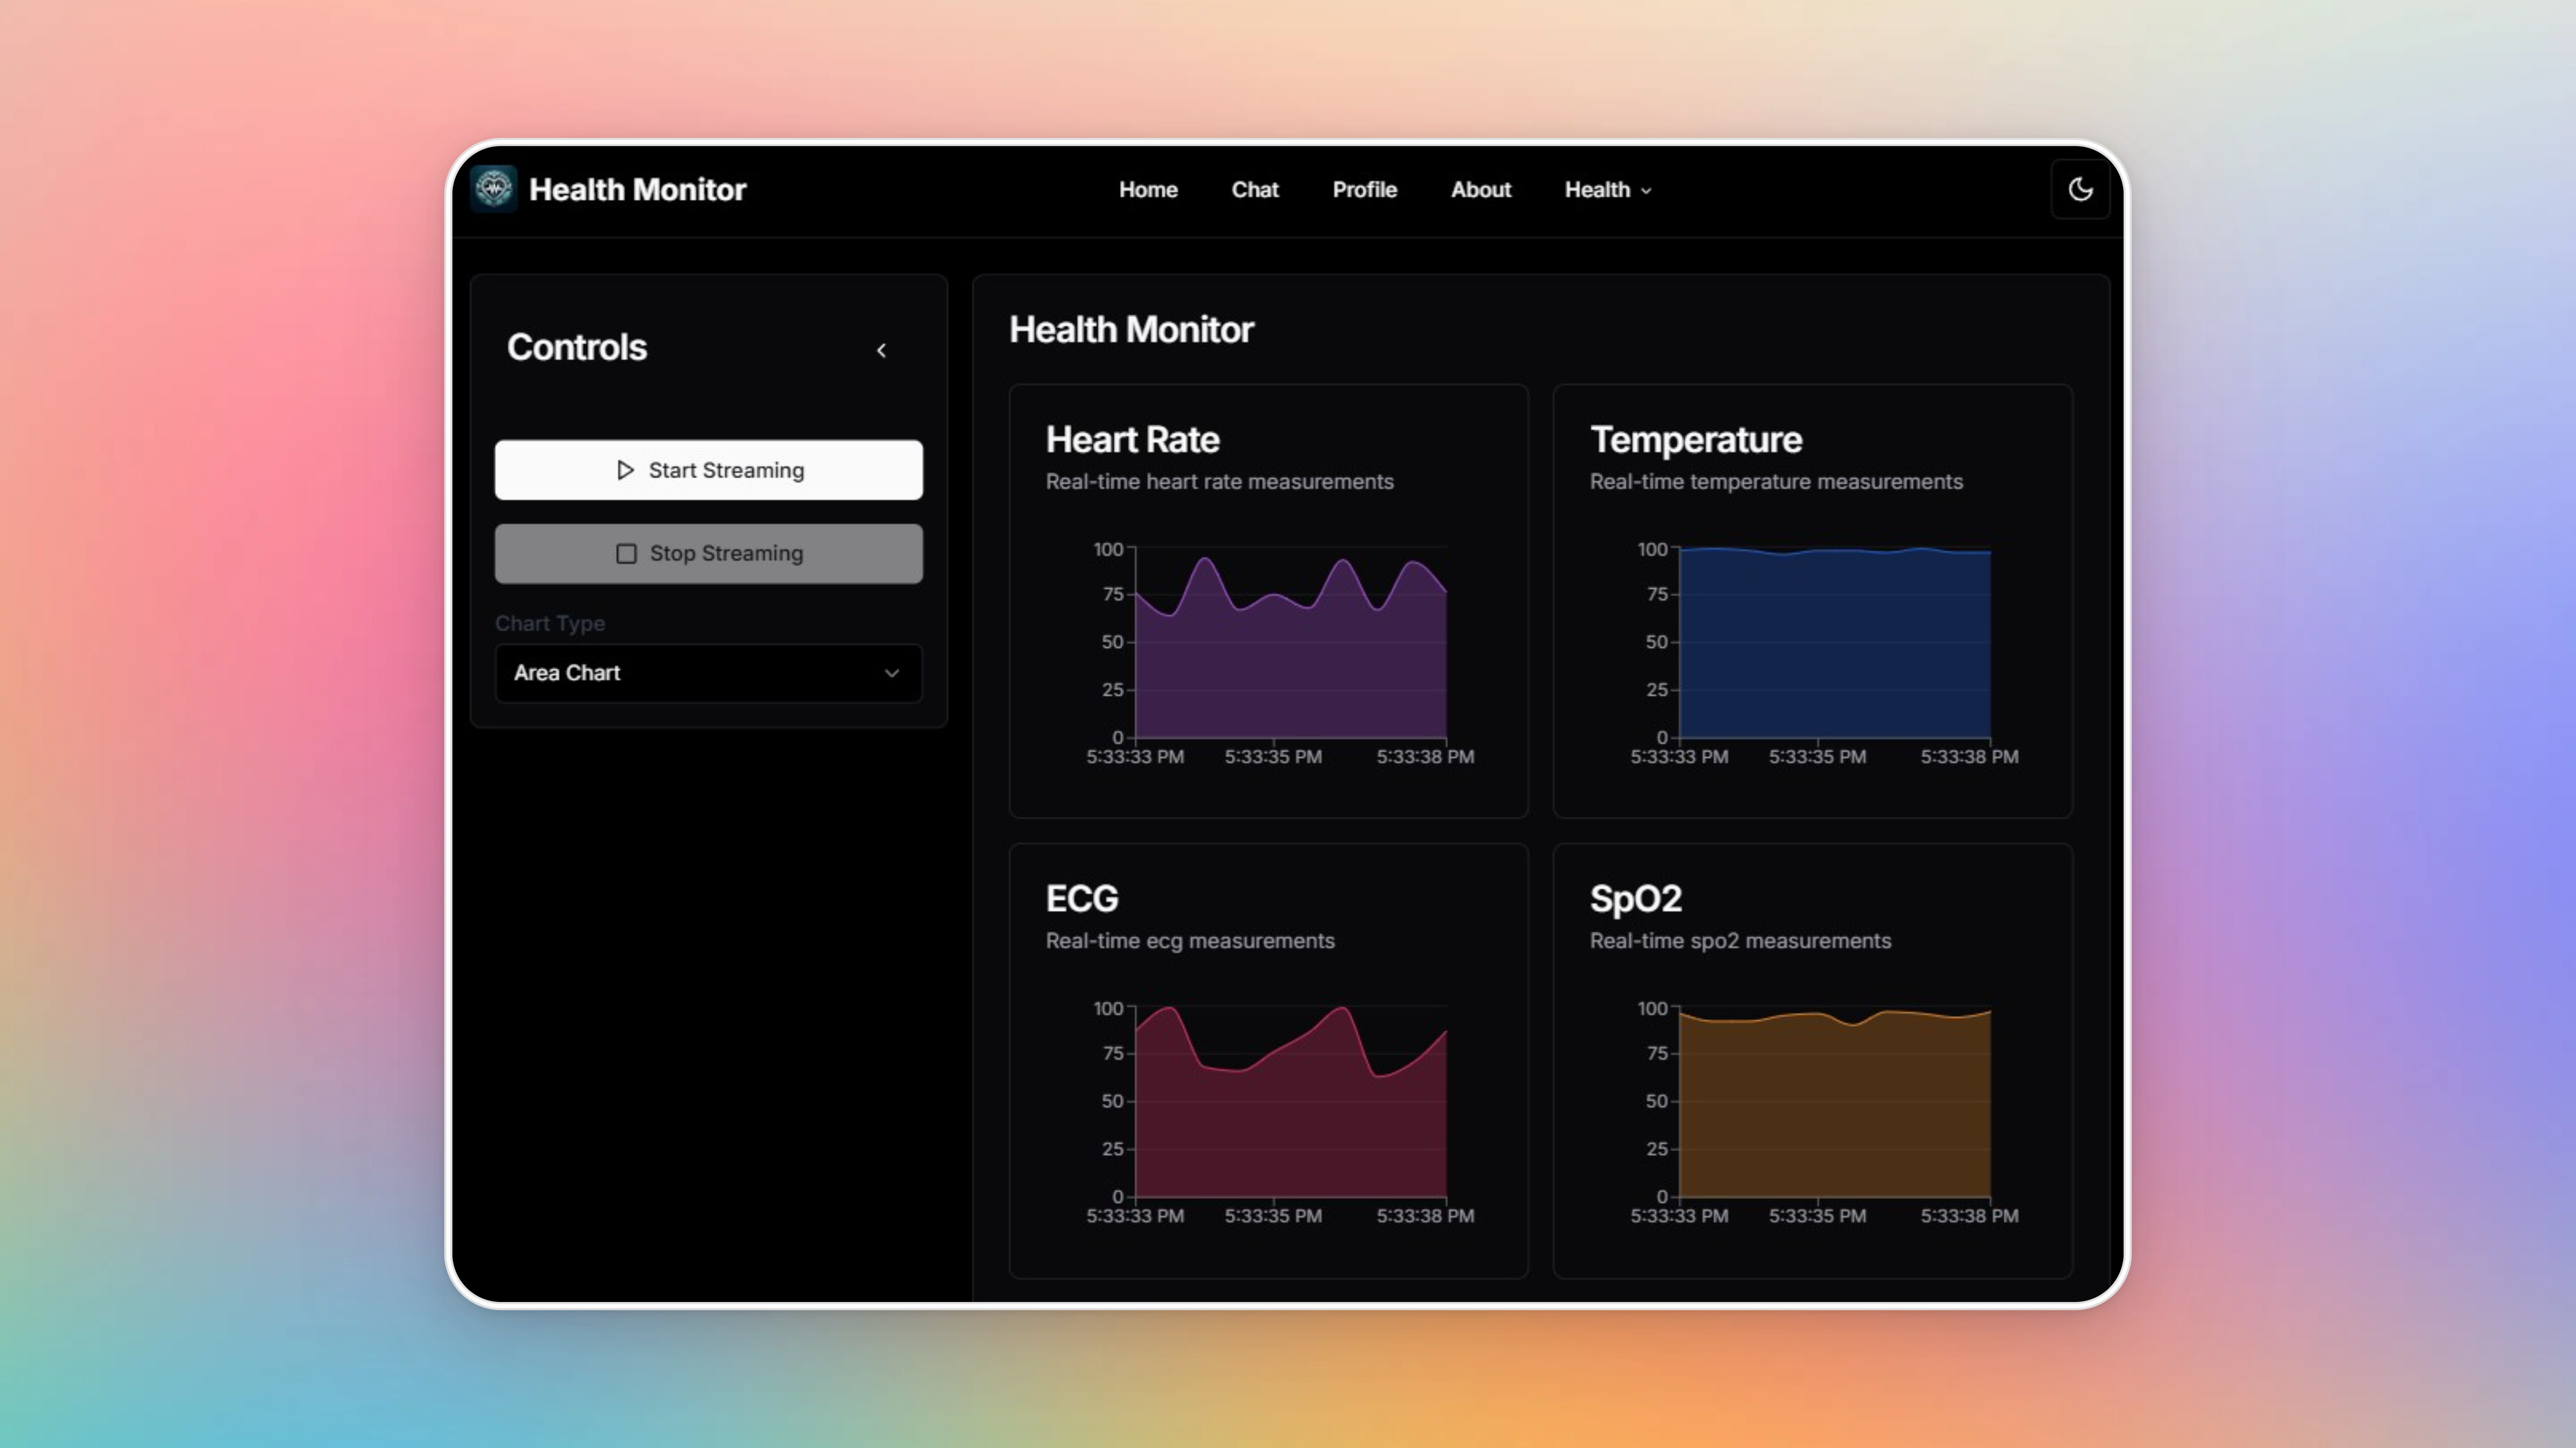
\includegraphics[width=0.8\textwidth]{images/hm-graphs.png}
    \caption{Health Analytics Dashboard}
\end{figure}

\subsection{Record Management}
\begin{figure}[H]
    \centering
    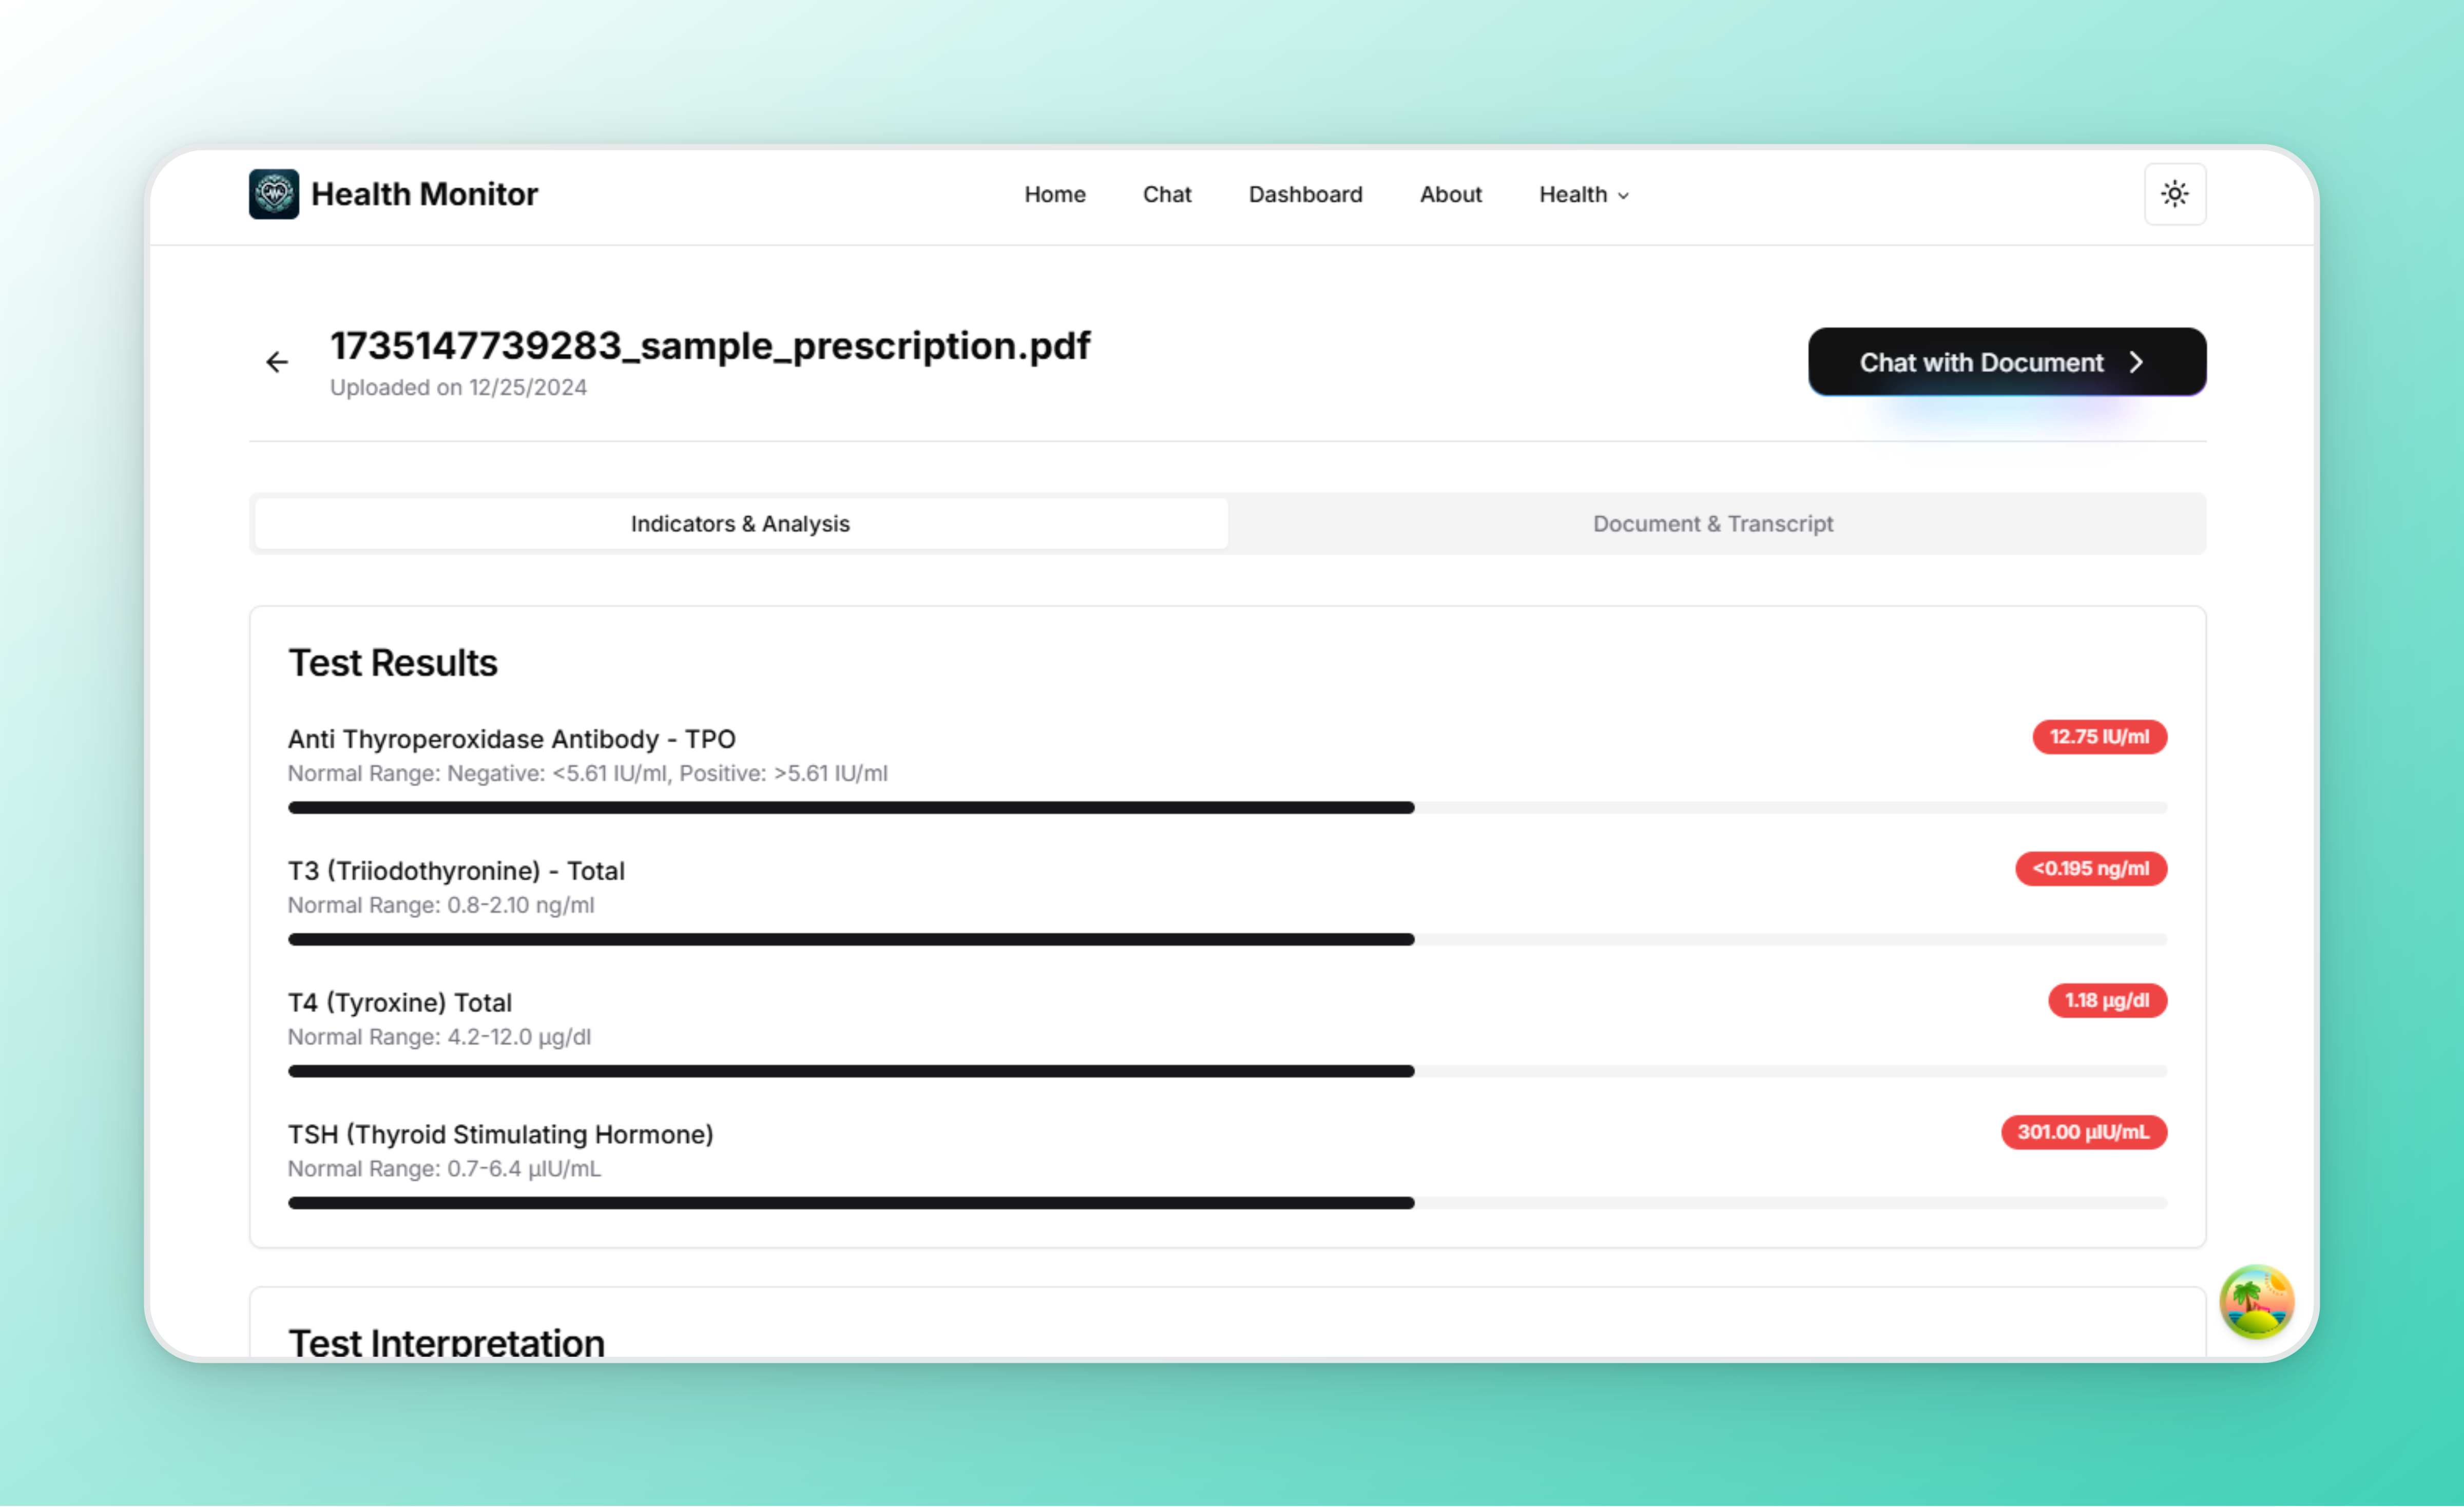
\includegraphics[width=0.8\textwidth]{images/hm-record-analysis.png}
    \caption{Health Record Analysis Interface}
\end{figure}

\section{System Architecture}
\subsection{Activity Monitoring}
\begin{figure}[H]
    \centering
    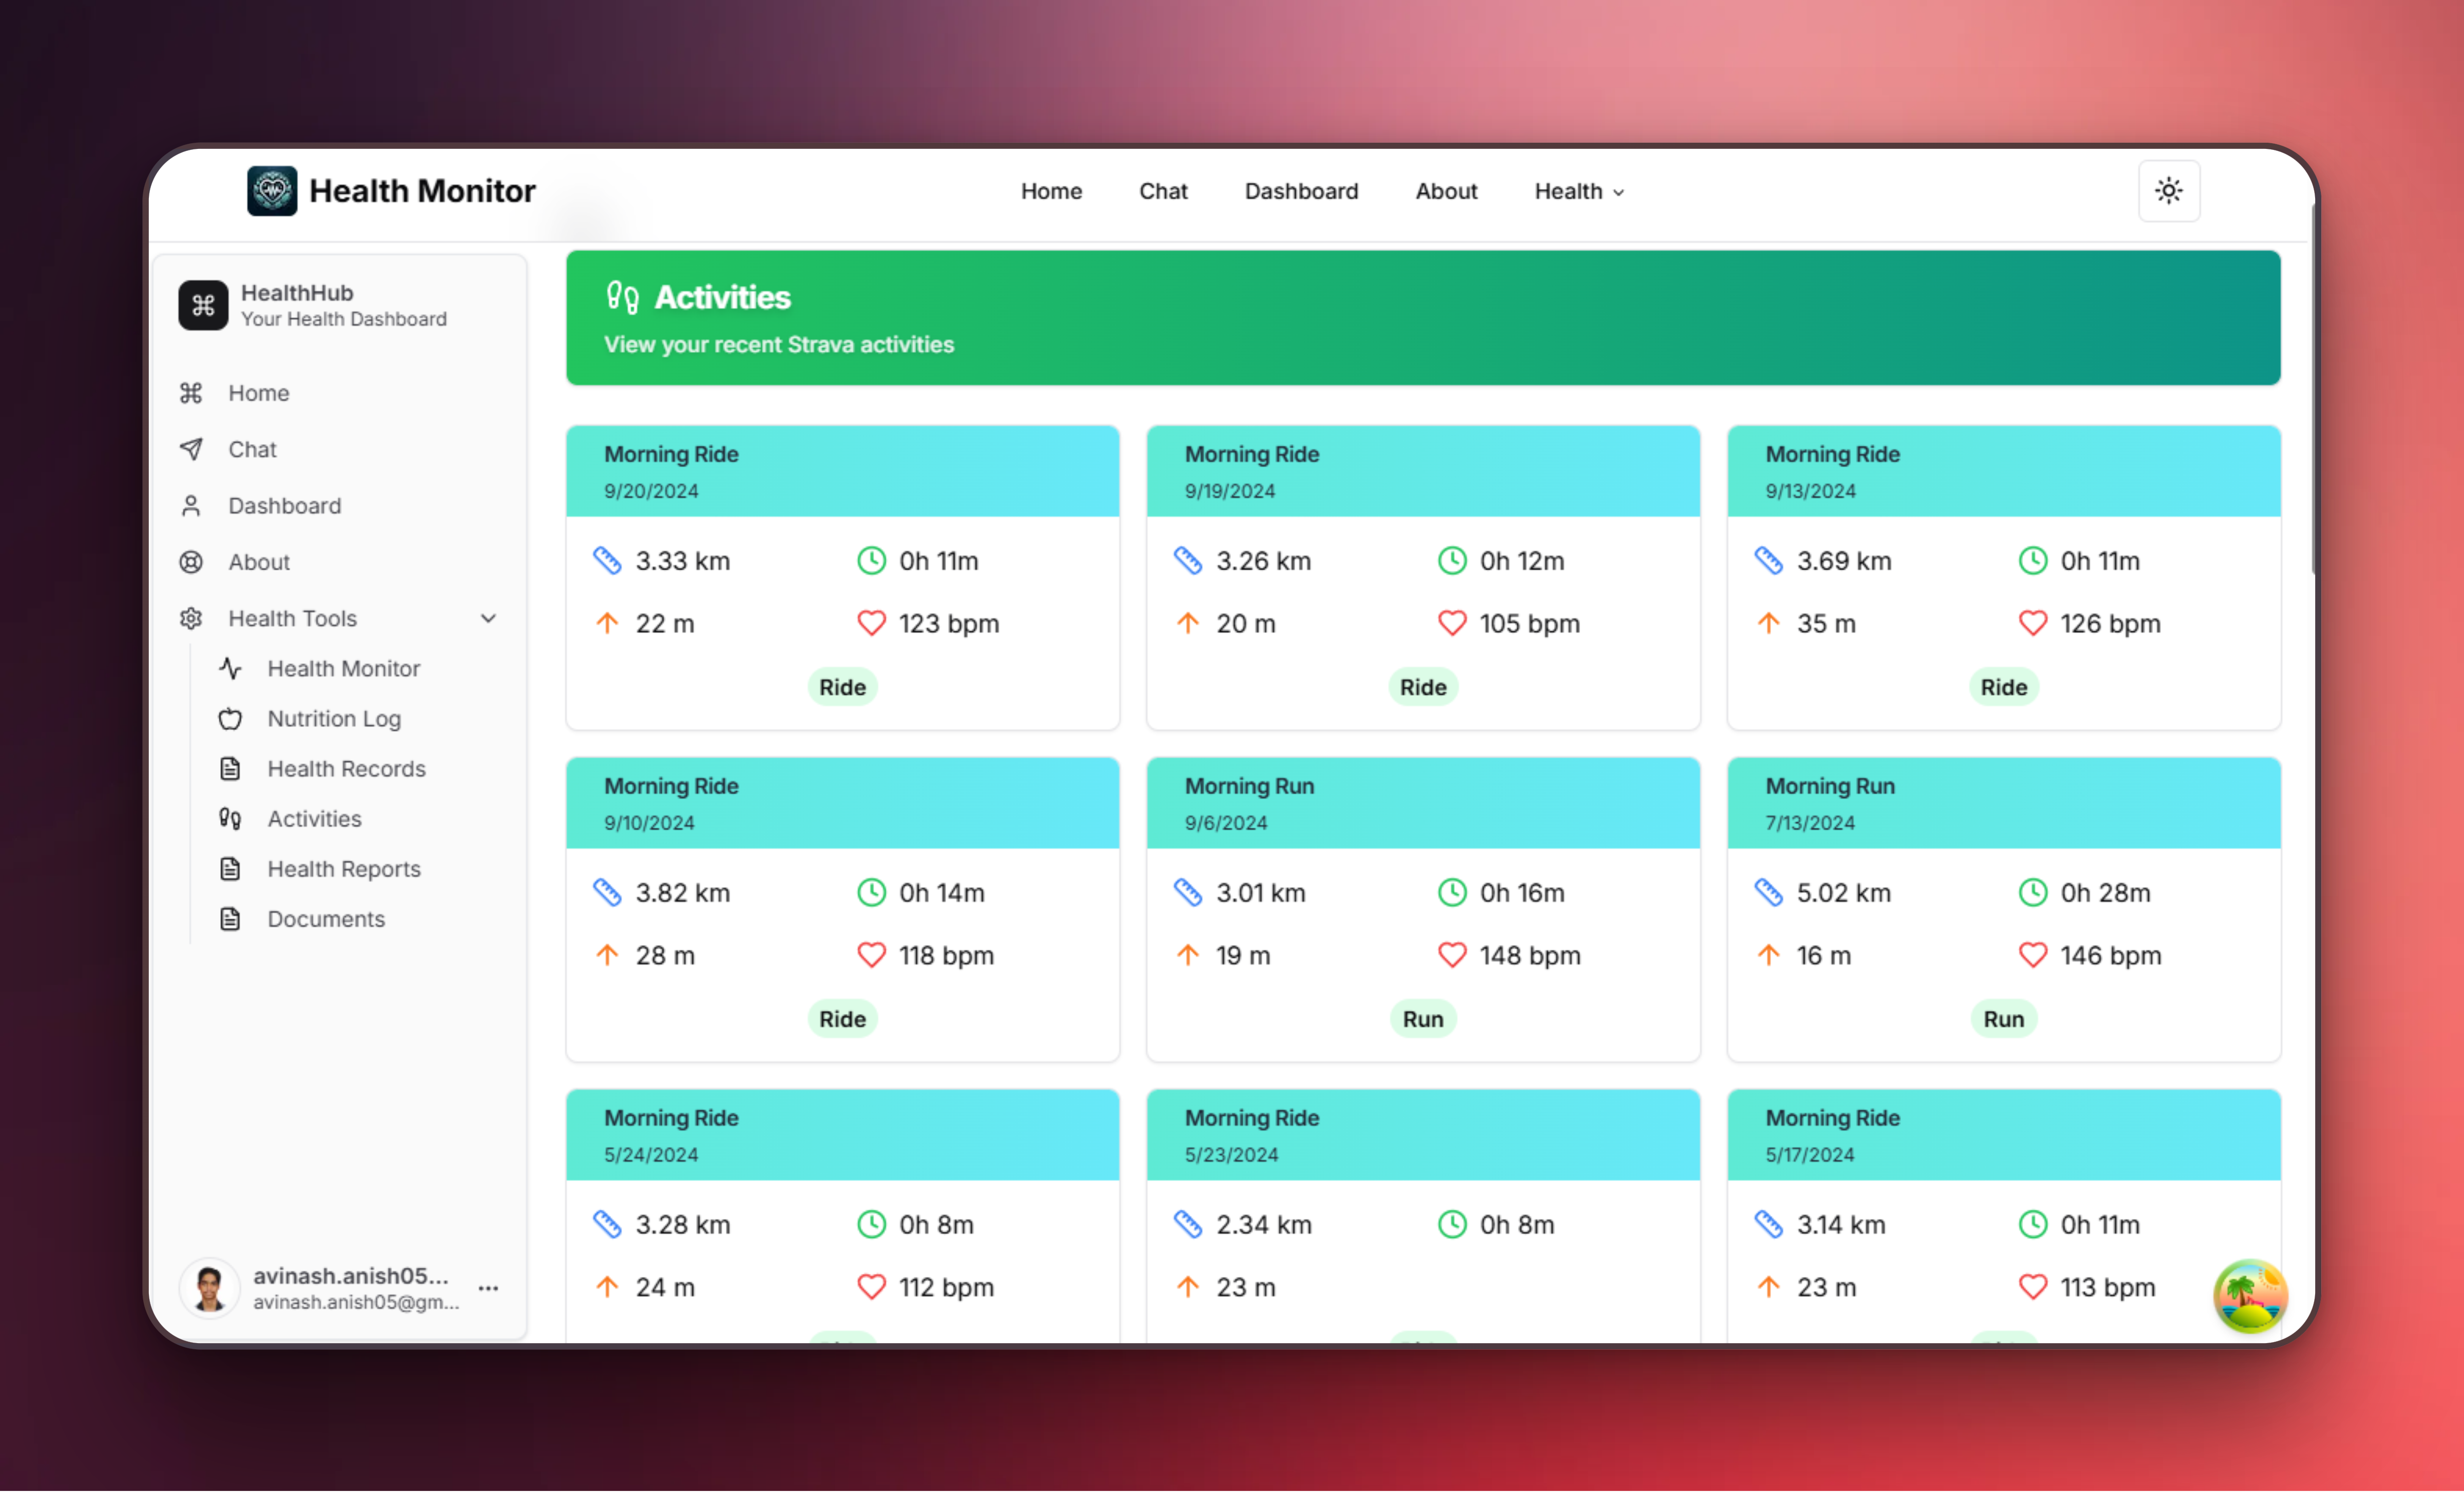
\includegraphics[width=0.8\textwidth]{images/hm-activities.png}
    \caption{Activity Tracking Interface}
\end{figure}

Each interface component was designed with user experience in mind, focusing on clarity, accessibility, and efficient information presentation. The implementation demonstrates the system's capability to handle various aspects of health data management, from real-time monitoring to detailed analysis and AI-assisted interpretation.

\newpage 